\chapter{SEGURANÇA DE REDE}

    Estar conectado à internet requer cuidados, pois dispositivos expostos à rede pública estão sujeitos às ameças de segurança que podem atacá-los. Sistema completamente seguro não existe, mas usuários finais devem tomar os devidos cuidados em suas redes locais bem como os ISPs também devem tomar as medidas cabíveis que estiverem ao alcance. No ISP, as competências de segurança atribuídas ao NOC são manter seguros os serviços, protocolos e as redes de telecomunicações, que estão nos níveis mais baixos da implementação das políticas de segurança da informação, enquanto o desenvolvimento de software e interação humano-computador estão em alto nível. A segurança é um acordo que deve ser cumprido por todas as partes em todos os níveis para minimização dos incidentes.

\section{IP Blacklist}

    A Minasnet, como sendo um AS, tem delegação de vários blocos de IP que darão aos seus assinantes identidade na internet. O primeiro problema quanto à segurança surge neste ponto, pois a conectividade traz riscos, que se iniciam pelo IP público, por onde os ataques conseguem propagar-se pela internet (ou pela intranet, via rede privada).
    
    Grande parte dos \textit{worms} são propagados pela internet através de \textit{spam}, que são enviados de maneira massiva por dispositvos infectados, sejam computadores, smartphones, roteadores domésticos e até roteadores de \textit{core}, basta ter conexão à internet que se torna vulnerável a \textit{botnets}. Assim, uma forma de controlar o envio de spam, por parte dos provedores de serviço, é a utilização de listas negras com IPs que são fontes de envio de \textit{spam}.
    
    Chamadas de \textit{Real-time Blackhole List} (RBL), doravante \textit{blacklist}, proporcionam a listagem de IPs detectados recentemente como participantes ativos de \textit{botnet} para envio de \textit{spam}, possibilitando ao provedor de serviço bloquear todo o tráfego de e-mail a partir daquele endereço IP listado. 
    
    Neste trabalho, o uso de RBL tem sua finalidade para monitoramento de IPs do AS listados na blacklist, com o objetivo de identificar infecções no core da rede, devido à vulnerabilidades associadas à equipamentos MikroTik com IP público, bem como nos assinantes. Para isso, foi utilizado o Composite Blocking List (CBL)\footnote{CBL, uma divisão da Spamhaus \url{https://www.abuseat.org}}, uma RBL com consula no padrão DNS Blacklist (DNSBL).
    
    DNSBL é informado pela RFC5782, funcionando com estrutura semelhante a um DNS reverso. Cada IP listado em uma DNSBL tem um subdomínio correspondente, sendo que cada entrada de subdomínio é criada revertendo os octetos do IP e concatenando com o domínio da DNSBL. Uma consulta à DNSBL retorna no registro {\tt A} o endereço 127.0.0.2 e no registro {\tt TXT} a descrição do motivo pelo qual o IP está listado na \textit{blacklist} \cite{rfc5782}. Quando o IP não está na \textit{blacklist}, a consulta retorna o erro {\tt NXDOMAIN}. Por exemplo, uma consulta para verificar se o IP 192.0.2.99 está listado na CBL seria feita a partir da entrada 99.2.0.192.cbl.abuseat.org e, em caso de listagem positiva, o link informado no registro {\tt TXT} daria um relatório detalhado da origem e qual tipo de infecção foi detectada atrás desse IP. Em terminal de comando Linux, a consulta pode ser feita da seguinte forma, para os registros {\tt A} e {\tt TXT}, respectivamente, conforme Figura \ref{fig:dnsbl_query}.
    
    \begin{figure}[!htb]
        \centering
        \caption{Exemplo de consulta à DNSBL CBL via terminal Linux.} 
        \label{fig:dnsbl_query}
        
        \begin{Verbatim}[fontsize=\small]
            host -t A 99.2.0.192.cbl.abuseat.org
            host -t TXT 99.2.0.192.cbl.abuseat.org
        \end{Verbatim} 

        {\small Fonte: do autor (2020).} 
    \end{figure}
    
    O monitoramento foi feito de maneira automatizada, através de um simples programa feito em Python para fazer a varredura de todos os blocos de IP do AS, que até o momento é constituído por 8.192 endereços. O programa varre todos os endereços o retorna relatório contendo somente aqueles listados na \textit{blacklist}, que são analisados com relatório detalhado na página da CBL.
    
    O Gráfico \ref{fig:plot_blacklist} mostra o resultado do monitoramento de IPs da Minasnet listados na CBL entre abril e setembro de 2019 e o Anexo A é um exemplo de relatório detalhado fornecido pela plataforma, contendo informações de origem, destino e tipo de infecção detectada pelo \textit{honeypot}, além de sugestões para correção do problema.
    
    \begin{grafico}[!htb]
        \centering
        \caption{Contagem de IPs do AS listados na CBL entre abril e setembro de 2019.} 
        \label{fig:plot_blacklist} 
        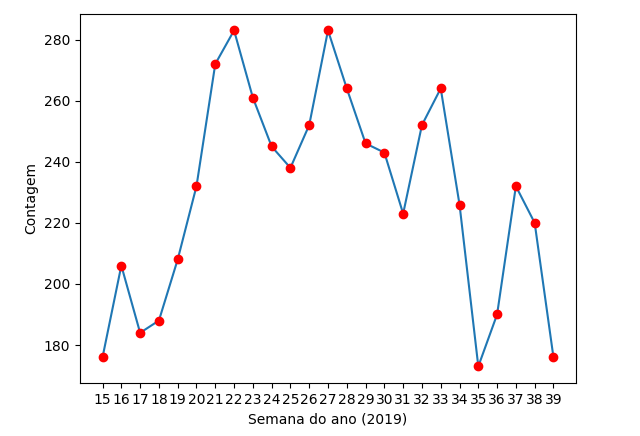
\includegraphics[scale=0.5]{img/plot_blacklist.png} \\
        {\small Fonte: do autor (2020).} 
    \end{grafico}
    
    \textit{Honeypots} são máquinas que emulam determinados sistemas operacionais e serviços, para que um atacante interaja com ela sem que perceba que está entrando em uma armadilha \cite{spampots2007}. É utilizando deste artifício que a CBL faz a detecção de \textit{botnets} e registra o IP de origem da fonte do \textit{spam}, sendo a Figura \ref{fig:honeypot} um exemplo de arquitetura utilizada para essa detecção. A descrição da metodologia utilizada pela plataforma pode ser obtida (em inglês) no site da CBL, já referenciado em nota de rodapé. 
    
    \begin{figure}[!htb]
        \centering
        \caption{Arquitetura de um honeypot para detecção de spam.} 
        \label{fig:honeypot} 
        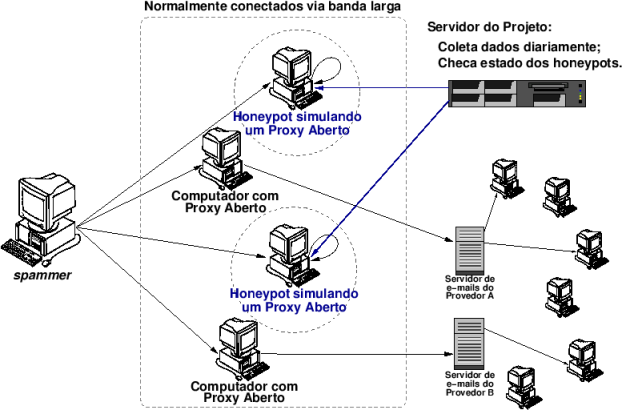
\includegraphics[scale=0.8]{img/honeypot.png} \\
        {\small Fonte: CERT.BR (2007).} 
    \end{figure}
    
    Apesar de o Gráfico \ref{fig:plot_blacklist} apresentar subidas e descidas acentudas na contagem dos IPs listados na \textit{blacklist}, não foi evidenciada nenhuma relação imediata entre a quantidade de IPs listados com as tratativas implementadas em firewall para tentar mitigar o problema, o que caracteriza que o \textit{spam} está originando-se da rede interna dos assinantes e trafegando na internet pela camada de aplicação, como pode ser visto no relatório apresentado no Anexo A, que relata a detecção através de tráfego HTTP. 
    
    A CBL oferece a opção de remoção manual de um IP listado, porém essa ação não soluciona o problema de fato, uma vez que caso a infecção ainda exista, muito provavelmente o IP retornará à listagem. Por isso, a melhor solução para o problema da \textit{blacklist} é a correção efetiva de vulnerabilidades existentes na rede, sendo que após um período de 28 dias sem nenhuma ocorrência, automaticamente o IP é removido da lista.

\section{Vulnerabilidades de rede}

    O CERT.br (Centro de Estudos, Resposta e Tratamento de Incidentes de Seguranca no Brasil) é responsável por tratar incidentes de seguranca computacional envolvendo redes conectadas à internet brasileira. Por isso, possui rotina de analisar, por amostragem, IPs registrados pelo Registro.br e notificar os responsáveis pelo AS no qual foi detectada alguma vulnerabilidade.
    
    Vulnerabilidades de rede são exploradas através de portas abertas em dispositivos, um vez que é pela camada que transporte que é possível estabelecer conexão e enviar pacotes pela rede. Portas de serviços mal configurados abertas são fonte para ataques de invasão, envio de \textit{spam} e DDoS (negação de serviço).
    
    Dessa forma, o CERT.br faz, regularmente, amostragem de IPs dos ASs brasileiros para realizar varredura de portas abertas, filtrando portas de serviços específicos que possam ser explorados por atacantes na internet e notificando as operadoras responsáveis. Uma varredura de portas, ou \textit{scan} de portas, pode ser feita a partir de terminal de comando pela ferramenta {\tt nmap}. Através do comando Figura \ref{fig:nmap}, pode ser feita a verredura de todas as portas do \textit{host} 192.0.2.99, por exemplo.

    \begin{figure}[!htb]
        \centering
        \caption{Exemplo de uso do nmap para varredura de portas.} 
        \label{fig:nmap} 
        
        \begin{Verbatim}[fontsize=\small]
            nmap -p- 192.0.2.99 -T5
        \end{Verbatim} 
        
        {\small Fonte: do autor (2020).} 
    \end{figure}
    
    Quando portas de serviços vulneráveis são detectadas como abertas, o CERT.br envia um e-mail contendo relatório detalhado da vulnerabilidade ao responsável pela administração daquele IP escaneado, além de forncer formas de corrigir o problema. O Anexo B é um e-mail enviado pelo CERT.br à Minasnet após detectar vulnerabilidade no protocolo SOCKS em dispositivos MikroTik na rede.
    
    As vulnerabilidades surgem devido a configuração errônea de CPEs por parte dos instaladores nas residências ou comércios, ou por parte dos analistas no núcleo da rede. 
    
    A correção dessas vulnerabilidades pode ser resolvida com a configuração correta de todos os equipamentos, difícil de ser atingido devido ao fator humano ser responsável pela garantia das configurações. Assim, a melhor tratativa necessita ter a menor dependência com humanos, sendo neste trabalho utilizada abordagem de firewall para filtragem de portas e VPN para controlar o acesso.
    
    A seguir são citadas algumas das vulnerabilidades de rede tratadas no firewall deste trabalho.
    
\subsection{Vulnerabilidade de obtenção de informação}
    
    São fontes de informações protocolos como SNMP e NetBIOS, além de banners de protocolos como Telnet e FTP, que aparecem após conexão ao servidor \cite{nakamura2007}. SNMP e NetBIOS são serviços que devem estar disponíveis apenas para LAN, não fazendo sentido estarem abertos na internet.

\subsection{Vulnerabilidade de acesso}

    São portas de entradas para atacantes invadirem o dispositivo, através de ataque de dicionário para advinhação de senhas por meio protocolos como Telnet, SSH, API e aplicações de gerenciamento, além reconfiguração de equipamentos através de SNMP.

\subsection{Vulnerabilidade de amplificação de ataque}

    São meios de atacantes de DDoS conseguirem amplificar o tráfego e congestionar a rede, explorando protocolos como DNS e SSDP, que têm o pacote de resposta muito maior que a requisição, podendo inundar a rede em um ataque coordenado. SSDP é um serviço de descoberta de LAN e por isso não tem sentido nenhum estar exposto à internet.

\section{Implementação de VPN}

    A abordagem do trabalho é primeiro filtrar o acesso implementando serviço de VPN e depois fazer a filtragem de portas. Para isso, foi adotado o OpenVPN\footnote{OpenVPN é uma VPN SSL open source \url{https://openvpn.net}}, por ser gratuito, portável para várias plataformas e ser possível customizá-la, pois é um serviço completo de VPN SSL que roda em um servidor Linux, podendo integrá-la com vários outros serviços e protolocos. VPNs L2TP/IPSec e PPTP não possuem tanto recursos e flexibilidade como OpenVPN suporta. Além disso, OpenVPN é um projeto open source, que conta com grande comunidade, documentação e fórum de suporte e discussão. OpenVPN também possui serviços prontos e pagos para empresas e para usuários finais.
    
    O projeto da VPN é bem simples, possuindo apenas dois requisitos: deve redar em um servidor único e possuir autenticação de dois fatores (2FA). Assim, o \textit{deploy} do servidor foi feito em uma VPS Debian Linux, mantida no datacenter da Minasnet, com as seguintes configurações de hardware:
    
    \begin{enumerate}[label=\alph*)]
        \item processador: Intel Xeon X7550;
        \item quantidade de núcleos: 2;
        \item memória RAM: 2GB;
        \item disco: 60GB;
        \item capacidade de rede: 1Gbps;
    \end{enumerate}
    
    A configuração do servidor foi feita inicialmente aplicando uma camada básica de segurança, seguindo o princípio do privilégio mínimo, deixando somente as portas necessárias abertas e restringindo o acesso SSH somente ao usuário administrador. Foi elaborado manual desse procedimento inicial e está disponível para consulta no Apêndice B.
    
    Aplicado o princípio do privilégio mínimo ao servidor base onde será implantada a VPN, foi feita a implantação do serviço OpenVPN, também sendo criado manual das configurações efetuadas, que está disponível no Apêndice C.
    
    A configuração do servidor OpenVPN consiste em criar uma infraestrutura de chave privada (PKI) utilizando da ferramenta de CLI EasyRSA\footnote{EasyRSA é um utilitário de CA (\textit{Certification Authority}) \url{https://github.com/OpenVPN/easy-rsa}}, responsável pela autoridade dos certificados SSL utilizados na VPN. É recomendado manter os servidores de PKI e de VPN em máquinas distintas (serviço de autenticação e de produção separados), entretanto para a finalidade deste trabalho foi mantido um servidor monolítico.
    
    Com a PKI operante, é feita as configurações do OpenVPN propriamente ditas, ajustando os parâmetros para funcionamento básico do serviço: permitir que usuários autentiquem-se via internet e acessem a intranet através do túnel.
    
    O sistema 2FA utiliza o certificado SSL, mantido pela PKI, e autenticação por usuário e senha, suportados pelo plugin PAM do Linux. A vantagem em utilizar PAM é a simplicidade de manutenção das contas de usuários, utilizando {\tt adduser} para criar um novo usuário, {\tt passwd} para alteração da senha e {\tt deluser} para remoção do usuário do sistema.
    
    Além disso, foi criado um \textit{script} feito em Python para facilitar a criação de usuários, ao invés de fazer manualmente via EasyRSA todas as vezes, como também cria os usuários de imediato. Não consiste em uma aplicação CLI totalmente funcional, apenas é um \textit{script} que facilita a chamada dos comandos de maneira automática, sendo que em caso de problemas, é demandado experiência em terminal de comando Linux para lidar com erros no EasyRSA, nas contas de usuários ou no gerenciador de serviços {\tt systemd}.
    
    Também é mantido um servidor OpenVPN de homologação, rodando em outra VPS e com PKI distinta, com a finalidade de efetuar testes de funcionalidades sem afetar o ambiente em produção.
    
    O ambiente em produção mantém conexão de dezenas de usuários simultaneamente sem perca de desempenho, servindo de porta de entrada à rede privada do provedor. A configuração atual permite que somente seja possível acessar equipamentos de núcleo da rede através da VPN, restringindo e controlando o acesso remoto a equipamentos críticos somente a usuários autorizados.
    
    O servidor OpenVPN principal está na rotina de backup automático das VPSs do datacenter da Minasnet, isso garante tolerância a falhas caso o servidor em produção corrompa, sendo somente necessário restauração de uma imagem do servidor que não seja perdido nenhum certificado da PKI, deste que o \textit{check-point} esteja em um instante após inserções de um novo usuário.
    
\subsection{Considerações sobre o servidor OpenVPN}

    A manutenção de um servidor OpenVPN demanda perícia em ambiente Linux, pois resolução de falhas requer análise de log do {\tt systemd}. Um detalhe é que o serviço da VPN não se inicia automaticamente quando o servidor é reiniciado por causa da necessidade de inserção manual do \textit{passphrase} da PKI em prompt no terminal de comandos.
    
    Outro detalhe é que os certificados SSL têm prazo de validade de 3 anos, sendo que não é possível simplesmente renovar a data de validade. É importante monitorar a validade dos certificados e gerar novos depois de vencidos para que não haja transtorno para os usuários da VPN.
    
\section{Implementação de firewall}

    Com a VPN operacional, o próximo passo para implementação de segurança na rede é a configuração de sistema de firewall para filtragem de pacotes suspeitos, com a finalidade de mitigar as vulnerabilidades elencadas pelas notificações do CERT.br bem como com políticas de segurança de rede adotadas pelo ISP.
    
    A abordagem de firewall deste trabalho é simples e eficiente, fazendo filtragem por endereços IP e por números de porta, ou seja, o firewall vai inspecionar pacotes na camada de rede e de transporte. Existem modelos de firewall que inspecionam pacotes na camada de aplicação (firewall \textit{layer} 7), porém requerem muito poder de processamento e podem afetar negativamente o \textit{throughput} da rede, sendo dedicados à redes corporativas (universidades e grandes corporações) ao invés de provedores de internet. Filtrar IP e porta é suficiente para a função do ISP.
    
    Antes da implantação deste trabalho, não existia firewall na rede de acesso dos clientes da Minasnet, ou seja, todos os CPEs dos clientes estavam expostos à internet sem nenhum filtro, sendo a única camada de segurança a manutenção de senhas fortes nos equipamentos e configuração correta por parte dos instaladores, algo que nem sempre ocorria. Houve relatos, por exemplo, de antenas Ubiquiti e MikroTik que foram infectadas por \textit{worms} devido às vulnerabilidades.
    
    Elencadas as vulnerabilidades nos quais os equipamentos de rede estão suscetíveis, a tarefa é implementar as regras de firewall e colocá-las em produção em um dispositivo que faça interface os tráfegos de rede. A abordagem deste trabalho utiliza do firewall nativo da plataforma RouterOS dos roteadores MikroTik, que possui seus fundamentos em iptables do Linux.
    
    Os requisitos de firewall desenvolvidos para a Minasnet, inicialmente, são os seguintes: 
    
    \begin{enumerate}[label=\alph*)]
        \item negar o acesso remoto aos equipamentos primários dos clientes, que desempenham a função de cliente PPPoE;
        \item permitir somente que o NOC e o Help Desk acessem remotamente os equipamentos dos clientes;
        \item permitir que clientes de IP fixo fiquem expostos à internet, sem filtragem por firewall;
        \item negar que clientes acessem a intranet do ISP;
        \item aplicar filtros que corrijam vulnerabilidades detectadas na rede.
    \end{enumerate}
    
\subsection{Firewall no RouterOS}

    O objetivo deste firewall é filtrar conexões de entrada que caracterizem como acesso ilegal a equipamentos, baseado em regras definidas por IP e porta. Filtrar consiste em descartar pacotes de acordo com as regras.
    
    A topologia utilizada para implantação do firewall aplica as regras diretamente ao concentrador, uma vez que é nele que está a origem (ou destino, dependendo do ponto de vista) do tráfego dos clientes. Colocar outro equipamento intermediando o concentrador com finalidade de firewall não é suficiente, pois não é possível filtrar conexões entre clientes de um mesmo concentrador de acordo com a metodologia utilizada neste trabalho.
    
    De acordo com a documentação do RouterOS \cite{fwmikrotik}, para implementar o firewall de acordo com os requisitos supracitados, é utilizado dos seguintes recursos oferecidos:
    
    \begin{enumerate}[label=\alph*)]
        \item {\tt address-list}: estrutura de dados do tipo lista contendo endereços que serão alvo das regras;
        \item {\tt action}: como o objetivo é filtrar, será utilizada como ação \textit{drop};
        \item {\tt chain}: como os pacotes que serão filtrados estão sendo roteados, utiliza-se da cadeia \textit{forward};
        \item {\tt protocol}: sendo TCP ou UDP;
        \item {\tt in-interface} ou {\tt out-interface}: sendo o alvos das regras, todos os clientes PPPoE;
        \item {\tt src-port} ou {\tt dst-port}: número de porta que serão filtradas pelo firewall.
    \end{enumerate}
    
    Não será exposto o script completo de configuração do firewall dos concentradores da Minasnet neste documento, por questão de segurança e de confidencialidade, uma vez que pessoas mal intencionadas poderiam explorar alguma vulnerabilidade que tenha passada despercebida na metodologia utilizada. Mesmo que não exista sistema 100\% seguro, mantendo confidencialidade é possível dificultar o trabalho dos atacantes. 
    
    A implantação de firewall no concentrador requer cuidado, uma vez que pode comprometer o desempenho da Routerboard. Por isso, foi feito monitoramento de consumo de CPU em diferentes horários do dia, inclusive em horários de pico por volta das 20h, para constatar que o firewall desenvolvido não afetou o desempenho do roteador consideravelmente, sendo que o processamento do concentrador já era concorrido pela manutenção das \textit{queues} e do CGNAT.
